%% The following is a directive for TeXShop to indicate the main file
%%!TEX root = diss.tex

\chapter{Stability Criteria and Performance Goals}
\label{ch:Stability}

Due to the nonlinear effects of the quantizer, the stability of the sigma delta feedback loop is difficult to prove. An excellent exploration into the mechanisms of instability may be found in \cite{Risbo1994}. There are no known necessary conditions for stability of sigma delta modulators but there are several heuristic and sufficient conditions with various degrees of conservativenenss. In \autoref{sec:stab-nl}, some theory from relay feedback control is introduced to establish formal methods for ensuring stability. There are some shortcomings of these methods when applied to practical sigma delta modulator design, therefore Sections~\ref{sec:stab-hinf} to \ref{sec:stab-l1} describe some stability criteria that may be less robust but allow a greater performance-stability tradeoff. For completeness, additional stability methods of interest that are not compatible with this optimization framework are presented in \autoref{sec:stab-notused}. Finally. the performance goal is discussed in \autoref{sec:stab-perf}.

\section{Stability Criteria Used by this Optimization Framework}
\label{sec:stab-used}

\subsection{Ideas from Nonlinear Control}
\label{sec:stab-nl}

An early theoretical treatment of nonlinear control is the circle criterion, which provides a graphical frequency domain method for evaluating the stability of a \gls{CT} Lur'e system. A Lur'e system is a simplified negative feedback loop consisting of a linear plant with a nonlinear element $\psi(\cdot)$ in the feedback path such as the one shown in \autoref{fig:lure-sys}. The transfer curve of the nonlinear element may be time-varying and even non-monotonic but is bounded by a sector condition, a set of two lines passing through the origin with slopes $k_1$, $k_2$ that bound the curve.

\begin{figure}
	\centering
	% Augmented Plant
	\begin{tikzpicture}[ampersand replacement=\&,scale=0.75, every node/.style={scale=0.75}]
	
		% Place nodes using a matrix
		\matrix (m1) at (0,0) [row sep=2.5mm, column sep=5mm, matrix anchor=center]
		{
			%-----------------------------------------------------------------------------------------------
			\node[dspnodeopen,dsp/label=left]			(m00) {$r$};			\&
			\node[dspadder,label={below left:$-$}]		(m01) {};			\&
			\node[dspfilter]						(m02) {$H_1$};		\&
			\node[coordinate]						(m03) {};			\& \\
			%-----------------------------------------------------------------------------------------------
			\node[coordinate]						(m10) {};			\&
			\node[coordinate]						(m11) {};			\&
			\node[dspsquare,label={above:$\psi(\cdot)$}]	(m12) {\RaisingEdge};	\&
			\node[coordinate]						(m13) {};			\& \\
			%-----------------------------------------------------------------------------------------------
		};
		
		\draw[dspconn] 	(m00) -- (m01);
		\draw[dspconn] 	(m01) to node[midway,above] {$e$} (m02);
		\draw[dspline] 	(m02) -- (m03);
		\draw[dspline] 	(m03) to node[midway,right] {$u$} (m13);
		\draw[dspconn] 	(m13) -- (m12);
		\draw[dspline] 	(m12) -- (m11);
		\draw[dspconn]	(m11) to node[midway,left] {$y$} (m01);
		
		\node[coordinate,label={left:$\psi(\cdot)$:}] (g0) at (4.6,0) {};
		\node[coordinate] 	(g1) at (6,-0.5) {};
		
		\begin{axis}[
			at={(g1)},
			anchor=center,
			grid=major,
			x=10mm, y=10mm, 
			axis x line=center, axis y line=center, 
			axis line style={latex-latex},
			ymin=-2, ymax=2, 
			xmin=-2, xmax=2,
			domain=-2:2,
			yticklabels={-2,,,,2}, ytick={-2,-1,0,1,2},
			xticklabels={-2,,,,2}, xtick={-2,-1,0,1,2},
			xlabel={$u$}, ylabel={$y$},
			x label style={at={(axis cs:1.25,0)},anchor=south},
			y label style={at={(axis cs:0,1.25)},anchor=west},
			]
			\addplot[domain=-2:2, solid, thick, black]
				 coordinates {(-2,-2) (-2,-1.5) (-1,-1.5) (-1,-0.5) (0,-0.5) (0,0.5) (1,0.5) (1,1.5) (2,1.5) (2,2)};
			\addplot[name path=fl,domain=-4:0,black] {1/2*x};
			\addplot[name path=fh,domain=0:4,black] {1/2*x};
			\path[name path=yaxisl] (axis cs:0,-2) -- (axis cs:0,0);
			\path[name path=yaxish] (axis cs:0,2) -- (axis cs:0,0);
			\addplot[fill=black,fill opacity=0.15] fill between[of=fl and yaxisl,softclip={domain=-4:0}];
			\addplot[fill=black,fill opacity=0.15] fill between[of=yaxish and fh,softclip={domain=0:4}];
			\node[coordinate] (c2) at (axis cs:0,2) {};
			\node[coordinate] (c1) at (axis cs:2,1) {};
		\end{axis}
		
		\node[coordinate,anchor=south,label={above:$y=k_2 u$}] (l2) at (c2) {};
		\node[coordinate,anchor=west,label={right:$y=k_1 u$}] (l1) at (c1) {};
		
	\end{tikzpicture}
	\caption{A Lur'e system (left) with the example nonlinear transfer curve of an infinite quantizer ($\Delta=1$) shown with a shaded sector bounded region (right).} \label{fig:lure-sys}
\end{figure}

\begin{thm}[Circle criterion {\cite[Sec. 7.1.1]{Khalil2002}}] \label{thm:circle}
	Given the Lur'e feedback system in \autoref{fig:lure-sys} where the denominator of $H_1(s)$ is Hurwitz and $\psi(t, \cdot)$ is a memoryless function sector bounded by $[k_1, k_2]$, the closed-loop system is globally asymptotically stable if one of the following cases is true:
	
	\begin{enumerate}
		\item Case $\psi \in [k_1, \infty):$ The inequality in \autoref{eq:circle-1} is satisfied. \label{it:circle-1}
		
		\begin{equation}
			\Re\left\{\frac{H_1(s)}{1 + k_1H_1(s)}\right\} > 0 \label{eq:circle-1}
		\end{equation}
		
		\item Case $\psi \in [k_1, k_2], \quad k_2 - k_1 > 0:$ The inequality in \autoref{eq:circle-2} satisfied.
		
		\begin{equation}
			\Re\left\{\frac{1 + k_2H_1(s)}{1 + k_1H_1(s)}\right\} > 0 \label{eq:circle-2}
		\end{equation}
	\end{enumerate}
\end{thm}

The graphical interpretation for the circle criterion\footnote{The circle criterion has different graphical interpretations for the cases where $k_1 < 0$ and where $H_1(s)$ has zeros in the open right half-plane, but these are omitted because they are not valid quantizer transfer curves or because nonminimum phase $H_1(s)$ are not considered here (see \cite[Sec. 7.1.1]{Khalil2002} for a full examination).} is that the Nyquist plot of $H_1(s)$ does not enter the disk passing through the points $-\frac{1}{k_1} + j0$ and $-\frac{1}{k_2} + j0$ if $0 < k_1 < k_2$. When $0 = k_1 < k_2$, the Nyquist plot must lie to the right of the vertical line $\Re\{s\} = -\frac{1}{k_2}$. If a single-bit quantizer is used as is the scope of this thesis, the sector bounds include the entire first and third quadrants. Case~\ref{it:circle-1} from Theorem~\ref{thm:circle} then applies and the Nyquist plot of $H_1(s)$ must lie entirely in the right half-plane. The optimization framework presented in \autoref{ch:Optimization} may be used with the circle criterion although with a single-bit quantizer, the method is too restrictive for practical use.

The Popov criterion in Theorem~\ref{thm:popov} is a slightly less conservative approach that restricts the problem to time-invariant nonlinearities. 

\begin{thm}[Popov criterion {\cite[Sec. 7.1.2]{Khalil2002}}] \label{thm:popov}
	Given the Lur'e feedback system in \autoref{fig:lure-sys} where the denominator of $H_1(s)$ is Hurwitz and $\psi(\cdot)$ is a time-invariant memoryless function sector bounded by $[0, k_2]$, the closed-loop system is globally asymptotically stable if there exists a scalar $\gamma \geq 0$ such that the following inequality is satisfied:
	
	\begin{equation}
		\frac{1}{k_2} + \Re\{H_1(j\omega)\} - \gamma\omega\Im\{H_1(j\omega)\} > 0 \quad \forall \omega \in [0, \infty).
	\end{equation}
\end{thm}

The graphical interpretation for this criterion is that the Popov plot of $\omega\Im\{H_1(j\omega)\}$ versus $\Re\{H_1(j\omega)\}$ remains to the right of a line passing through point $-\frac{1}{k_2} + j0$ with slope $\frac{1}{\gamma}$. 

The \gls{DT} version is the Tsypkin criterion, which has cases valid for time-varying and time-invariant nonlinearities. The analog to the circle criterion is shown in Theorem~\ref{thm:tsypkin-1} and the analog to the Popv criterion is shown in Theroem~\ref{thm:tsypkin-2}.

\begin{thm}[Tskypin criterion for time-varying nonlinearities {\cite[Sec. 4.6]{Tsypkin1984}}] \label{thm:tsypkin-1}
	Given the Lur'e feedback system in \autoref{fig:lure-sys} where the denominator of $H_1(z)$ is Schur and $\psi(t,\cdot)$ is a memoryless function sector bounded by $[0, k_2]$, the closed-loop system is globally asymptotically stable if the following inequality is satisfied:
	
	\begin{equation}
		\frac{1}{k_2} + \Re\{H_1(z)\}\geq 0 \quad \forall |z| = 1.
	\end{equation}
\end{thm}

\begin{thm}[Tskypin criterion for time-invariant nonlinearities {\cite[Sec. 4.7]{Tsypkin1984}}] \label{thm:tsypkin-2}
	Given the Lur'e feedback system in \autoref{fig:lure-sys} where the denominator of $H_1(z)$ is Schur and $\psi(\cdot)$ is a time-invariant memoryless function sector bounded by $[0, k_2]$, the closed-loop system is globally asymptotically stable if there exists a scalar $\gamma \geq 0$ such that the following inequality is satisfied:
	
	\begin{equation}
		\frac{1}{k_2} + \Re\left\{\left(1 + \gamma\left(1 - z^{-1}\right)\right)H_1(z)\right\}\geq 0 \quad \forall |z| = 1.
	\end{equation}
\end{thm}

 The Jury-Lee criteria are less strict cases of the Tsypkin criteria requiring that the nonlinearity be slope bounded and monotonic. However, this is not applicable to quantizer feedback, where the slope may be infinite at points. The above techniques from nonlinear control are sufficient conditions and are related to important results from passivity theorem.
 
 \subsection{\gls{Hinf} Stability Criterion}
 \label{sec:stab-hinf}
 
The \gls{Hinf} stability criterion, commonly known as Lee's rule, is a heuristic predictor of stability stating that a modulator is likely to be stable if the \gls{NTF} out-of-band gain, or $||S(\lambda)||_\infty$, does not exceed a benchmark value. The rule was initially based on the empirical study of a fourth-order \gls{DT} sigma delta modulator with single-bit quantization \cite{Chao1990}. The criterion is not necessary nor sufficient for stability and must be verified with extensive simulations. Despite this, the rationale for its use as a suggestion of stability comes from the Bode sensitivity integral shown in \autoref{eq:bodeint-dt} for Schur stable $H_1(z)$ \cite[Thm. 1]{Zhao2015}.

\begin{equation} 
	\frac{1}{2\pi}\int_{-\pi}^{\pi} \log \left|S(\omega)\right|d\omega = 0 \label{eq:bodeint-dt}
\end{equation}

The integral enforces that the total area under the curve of the \gls{NTF} log-magnitude versus frequency is equal to zero. Applied to the sigma delta linear model, if the sensitivity of the closed-loop system to the quantization error is suppressed in the signal band, it must be compensated for by an equal area of amplified sensitivity outside the signal band. Because the quantization error is nonlinear and signal dependent, the higher the gain of the sensitivity function, the greater chance there is for a limit cycle at that frequency to destabilize the loop. Thus, the Lee's rule is a indicator of the performance-stability tradeoff. In practice, $||S(z)||_\infty \leq 2$ is often used, but this has been found to be conservative for low-order and inadequate for high-order designs \cite{Schreier1993}. However, the criterion is used extensively as a starting point for practical design due to its inclusion in popular software tools. A recent extension of Lee's rule produces a more complex \gls{Hinf} bound based on empirical results that may be used as an alternative stability goal \cite{Neitola2017}. This stability criterion is easy to formulate as part of an optimization problem as it may be applied with an \gls{Hinf} constraint on the $r \rightarrow e$ channel of \autoref{eq:aug}:

\begin{equation}
	||G_{er}(\lambda)||_\infty \leq \gamma_\infty. \label{eq:hinf}
\end{equation}
 
\subsection{Describing Function Approximation and Root Locus Stability}
\label{sec:stab-rl}

Two closely related stability methods are the describing function approximation and the root locus approach. These both rely on the variable gain \gls{K} introduced in \autoref{sec:model-linq} but use different interpretations of it to stabilize the modulator.

\begin{figure}
	\centering
	\begin{tikzpicture}[ampersand replacement=\&,scale=0.75, every node/.style={scale=0.75}]
		% Place nodes using a matrix
		\matrix (m0) at (0,2) [row sep=2.5mm, column sep=5mm, matrix anchor=west]
		{
			%-----------------------------------------------------------------------------------------------
			\node[coordinate]					(m0-0) {};				\&
			\node[dspsquare,dsp/label={above:$\psi$}]	(m0-1) {\RaisingEdge};		\&
			\node[dspnodeopen,dsp/label=right]		(m0-2) {$y$};			\& \\
			%-----------------------------------------------------------------------------------------------
		};
		% Place nodes using a matrix
		\matrix (m1) at (0,0) [row sep=2.5mm, column sep=5mm, matrix anchor=west]
		{
			%-----------------------------------------------------------------------------------------------
			\node[coordinate]					(m1-0) {};				\&
			\node[dspgain,fill=white]				(m1-1) {$\frac{2\Delta_Q}{\pi A}$};	\&
			\node[dspnodeopen,dsp/label=right]		(m1-2) {$\hat{y}$};		\& \\
			%-----------------------------------------------------------------------------------------------
		};
		
		\begin{pgfonlayer}{bg}
			\draw[->]	($(m1-1) + (-0.5,-0.5)$) -- ($(m1-1) + (0.5,0.5)$);
		\end{pgfonlayer}
		
		%\draw[dspconn]	(m0-0) -- (m0-1);
		\draw[dspconn]	(m0-1) -- (m0-2);
		%\draw[dspconn]	(m1-0) -- (m1-1);
		\draw[dspconn]	(m1-1) -- (m1-2);
		\node[rotate=90] at (1.4,1) {$\approx$};
		\node[coordinate] 	(g0) at (-2.75,1) {};
		\node[dspnodeopen,label={left:$u$}] 	(g1) at (-1,1) {};
		\node[dspnodefull]	(g2) at (0,1) {};
		\coordinate		(m0-0x) at (g2 |- m0-0);
		\coordinate 		(m1-0x) at (g2 |- m1-0);
		\draw[dspline]	(g1) -- (g2);
		\draw[dspline]	(g2) -- (m0-0x);
		\draw[dspline]	(g2) -- (m1-0x);
		\draw[dspconn]	(m0-0x) -- (m0-1);
		\draw[dspconn]	(m1-0x) -- (m1-1);
		\node[coordinate]	(g3) at ($(m0-2) + (1.75,0)$) {};
		
		% Analog signal.
		\begin{axis}[
			at={(g0)},
			anchor=center,
			x=12mm, y=6mm, 
			axis x line=center, axis y line*=left, 
			ymin=-1, ymax=1, 
			yticklabels={}, xticklabels={},
			xlabel={}, ylabel={$A\sin(\omega t)$},
			x label style={at={(axis cs:1,0)}, anchor=east},
			y axis line style={draw=none},
			tick style={draw=none}
			]
		\addplot[domain=-0:2,smooth,thick, black]
			plot {sin(deg(2*pi*x))};
		\end{axis}
		
		% Analog signal.
		\begin{axis}[
			at={(g3)},
			anchor=west,
			x=12mm, y=6mm, 
			axis x line=center, axis y line*=left, 
			ymin=-1, ymax=1, 
			xticklabels={},
			yticklabels={$-\frac{\Delta_Q}{2}$,$\frac{\Delta_Q}{2}$}, ytick={-1,1},
			xlabel={}, ylabel={$\frac{\Delta_Q}{2}\textrm{sign}(u)$},
			x label style={at={(axis description cs:1,0)}, anchor=east},
			y axis line style={draw=none},
			tick style={draw=none}
			]
		\addplot[domain=-0:2, thick, black]
			coordinates{(0,0) (0,1) (0.5,1) (0.5,-1) (1,-1) (1,1) (1.5,1) (1.5,-1) (2,-1) (2,0)};
		\end{axis}
		
	\end{tikzpicture}
	\caption{An ideal 1-bit quantizer (above) and its describing function approximation (below).} \label{fig:df}
\end{figure}

The describing function method \cite{Taylor1999} is an approximate technique of linearization often applied to steady-state electrical circuits or to nonidealities in mechanical systems. As shown in \autoref{fig:df}, a zero-mean sinusoidal input to the quantizer is assumed: $u(t) = A\sin(\omega t)$. The Fourier series of the output is truncated at the first odd coefficient because the quantizer transfer curve is also an odd function. For a single-bit quantizer, the first coefficients are:

\begin{align}
	a_1 &= \frac{1}{\pi} \int_0^{2\pi} \psi(t)\cos(\omega t) d(\omega t) \label{eq:fourier-a} \\
	b_1 &= \frac{1}{\pi} \int_0^{2\pi} \psi(t)\sin(\omega t) d(\omega t), \label{eq:fourier-b}
\end{align}

where $\psi(t)$ is the nonlinear quantizer function. Integral~\ref{eq:fourier-a} evaluates to zero while the period of Integral~\ref{eq:fourier-b} may be split into two parts:

\begin{equation*}
	b_1 = \frac{1}{\pi}\left(\int_0^\pi\psi(t)\sin(\omega t)d(\omega t) + \int_\pi^{2\pi}\psi(t)\sin(\omega t)d(\omega t)\right).
\end{equation*}

In the interval $\omega t \in (0, \pi)$, the single-bit quantizer outputs $\frac{\Delta_Q}{2}$ whereas in the interval $\omega t \in (\pi, 2\pi)$, the single-bit quantizer outputs $-\frac{\Delta_Q}{2}$. By symmetry, this integral simplifies to \autoref{eq:df-derivation}.

\begin{equation}
	b_1 = \frac{\Delta_Q}{\pi}\int_0^\pi \sin(\omega t)d(\omega t) = \frac{2\Delta_Q}{\pi} \label{eq:df-derivation}
\end{equation}

Using the Fourier series approximation $\hat{y}(t) \approx y(t)$, the describing function is derived as follows:

\begin{align*}
	K(A) &= \frac{\hat{y}(t)}{u(t)} \\
	&= \frac{b_1\sin(\omega t)}{A\sin(\omega t)} \\
	&= \frac{2\Delta_Q}{\pi A}.
\end{align*}

Thus, the describing function of the single-bit quantizer is a variable gain \gls{K(A)} dependent on the quantizer input amplitude. As expected, when the input amplitude approaches zero, the gain approaches infinity and when it approaches $\pm\frac{\Delta_Q}{2}$, the gain approaches one. In fact, instability in sigma delta modulators is often associated with low frequency, large amplitude limit cycles where the quantizer gain is low. The describing function method is a good approximation to large signal stability but often fails to predict small limit cycles because the higher harmonics of the output are neglected. The describing function has been applied to the design of sigma delta modulators \cite{Engelen1999} and extended to be dependent on phase in addition to gain to design a sixth-order modulator \cite{VanEngelen1999a}.

In the open loop, the describing function method approximated the quantizer as a variable gain. The root locus can determine stability by showing the position of the closed-loop poles as a function of this gain. One method to design stable sigma delta modulators is to position the poles and zeros of the loop filter such that the root locus remains in the stable region of the complex plane when sweeping through valid quantizer gain values \cite{Yang2002, Kuo2006, Kang2014}. Recall that the \gls{LFT} was used to model the varying gain in \autoref{sec:model-lft}. \autoref{eq:lft-range} defines \gls{M} when the gain is within a given range $K \in [k_l, k_h]$ with nominal value $k_0$.

\begin{equation}
	M = 
	\begin{bmatrix}
		\frac{k_h - 2k_0 + k_l}{k_h - k_l} & \frac{-2(k_0 - k_h)(k_0 - k_l)}{k_h - k_l} \\
		1 & k_0
	\end{bmatrix}  \label{eq:lft-range}
\end{equation}

The root locus stability criterion may be used in robust control fashion by choosing a range for $K$, e.g. $[k_l, k_h] = [1/||u||_\infty, \infty]$, then constraining the \gls{Hinf} norm to unity for the $z \rightarrow w$ channel as seen in \autoref{eq:rl}. This ensures that the linearized model is stable for the selected gain values.
 
 \begin{equation}
 	||G_{zw}(\lambda)||_\infty \leq 1. \label{eq:rl}
 \end{equation}
 
 \subsection{\gls{H2} Stability Criterion}
 \label{sec:stab-h2}
 
 \begin{figure}
	\centering
	% Augmented Plant
	\begin{tikzpicture}[ampersand replacement=\&,scale=0.75, every node/.style={scale=0.75}]
	
		% Place nodes using a matrix
		\matrix (m1) at (0,0) [row sep=2.5mm, column sep=5mm, matrix anchor=center]
		{
			%-----------------------------------------------------------------------------------------------
			\node[coordinate]						(m00) {};			\&
			\node[coordinate]						(m01) {};			\&
			\node[coordinate]						(m02) {};			\&
			\node[dspnodeopen,dsp/label=above]			(m03) {\gls{meanu}};		\&
			\node[coordinate]						(m04) {};			\&
			\node[dspnodeopen,dsp/label=above]			(m05) {$d[k]$};		\&
			\node[dspnodeopen,dsp/label=above]			(m06) {\gls{meany}};		\&
			\node[coordinate]						(m07) {};			\& \\
			%-----------------------------------------------------------------------------------------------
			\node[dspnodeopen,dsp/label=left]			(m10) {$r[k]$};		\&
			\node[dspadder,label={below left:$-$}]		(m11) {};			\&
			\node[dspfilter]						(m12) {$H_1(z)$};		\&
			\node[dspadder,label={above right:$-$}]		(m13) {};			\&
			\node[dspgain,fill=white]					(m14) {$K$};			\&
			\node[dspadder]						(m15)	{};			\&
			\node[dspadder]						(m16)	{};			\&
			\node[dspnodefull]						(m17) {};			\&
			\node[dspnodeopen,dsp/label=right]			(m18)	{$y[k]$};		\& \\
			%-----------------------------------------------------------------------------------------------
			\node[coordinate]						(m20) {};			\&
			\node[coordinate]						(m21) {};			\&
			\node[coordinate]						(m22) {};			\&
			\node[coordinate]						(m23) {};			\&
			\node[coordinate]						(m24) {};			\&
			\node[coordinate]						(m25) {};			\&
			\node[coordinate]						(m26) {};			\&
			\node[coordinate]						(m27) {};			\& \\
			%-----------------------------------------------------------------------------------------------
		};
		
		\begin{pgfonlayer}{bg}
			\draw[->]	($(m14) + (-0.5,-0.5)$) -- ($(m14) + (0.5,0.5)$);
		\end{pgfonlayer}
		
		\draw[dspconn]	(m03) -- (m13);
		\draw[dspconn] 	(m05) -- (m15);
		\draw[dspconn] 	(m06) -- (m16);
		\draw[dspconn] 	(m10) -- (m11);
		\draw[dspconn]	(m11) to node[midway,above] {$e[k]$} (m12);
		\draw[dspconn] 	(m12) to node[midway,above] {$u[k]$} (m13);
		\draw[dspconn] 	(m13) -- (m14);
		\draw[dspconn] 	(m14) -- (m15);
		\draw[dspconn] 	(m15) -- (m16);
		\draw[dspconn] 	(m16) -- (m18);
		\draw[dspline] 	(m17) -- (m27);
		\draw[dspline] 	(m27) -- (m21);
		\draw[dspconn] 	(m21) -- (m11);
		
		\draw[Gray, ->, out=45, in=135, looseness=1] ($(m05)+(0.35, 0.55)$) to node[above, xshift=5pt] {$S(z)$} ($(m18)+(0.25, 0.35)$);
		
	\end{tikzpicture}
	\caption{The block diagram for the \gls{H2} stability criterion.} \label{fig:h2-block}
\end{figure}
 
 Previously, the quantizer was replaced by an additive noise source and some performance estimations were presented assuming that the quantization noise was uncorrelated with input had a white spectrum. The white noise model is only a close approximation if the following hold \cite[Ch. 6]{Gray1990}:
 
 \begin{enumerate}
 	\item The quantizer is not overloaded,
 	\item There are a large number of quantization levels with small \gls{delta}, and
 	\item The \gls{PDF} of input samples is smooth.
 \end{enumerate}
 
 In reality, especially with single-bit quantization, the approximation does not hold. The \gls{H2} stability criterion, sometimes called the power gain rule, uses a statistical look at the quantizer input \cite{Risbo1994}. The output $y[k]$ of a single-bit quantizer may be considered the superposition of three signals: a DC component \gls{meany}, AC component amplified by the quantizer gain $K\left(u[k] - \mu_u\right)$, and the quantization noise $d[k]$, as seen in \autoref{fig:h2-block}. With these additional degrees of freedom, one can enforce that $d[k]$ is zero mean, white, and uncorrelated with the quantizer input $u[k]$ by setting \gls{K} to that in \autoref{eq:h2-k1}.
 
 \begin{equation}
 	K = \frac{\cov\{u[k], y[k]\}}{\sigma_u^2} \label{eq:h2-k1} \\
 \end{equation}
 
 The gain \gls{K} is now entirely dependent on \gls{meany} and the distribution of \gls{u}. Due to the fact that $y[k]$ has bounded output power (equal to one with $\Delta_Q=2$ single-bit quantization), the variance at the output may be calculated:
 
 \begin{equation}
 	\sigma_y^2 = K^2\sigma_u^2 + \sigma_d^2.
 \end{equation} 
 
Functions relating \gls{meany} to \gls{vard} have been derived for the Gaussian \cite[Eq. 26]{Ardalan1987}, uniform \cite[Eq. 6.16]{Risbo1994}, and triangular \cite[Eq. 6.17]{Risbo1994} distributions. Once a distribution has been chosen, the only free variable remaining is \gls{meany}. 

With reference to \autoref{fig:h2-block}, the \gls{NTF} is the gain from quantization noise to the output. Because the \gls{H2} norm is a power gain, $||S(z)||_2^2$ is the amplification of variances \gls{vard} to \gls{vary}. Altogether, \gls{meany} defines \gls{vard}, so for bounded output power, a maximum $||S(z)||_2$ is established. The \gls{H2} stability criterion can be applied by choosing a quantizer input signal distribution, which sets the relationship between \gls{meany} and $||S(z)||_2$. Because the \gls{STF} gain is near one in the signal band, \gls{meany} tracks input $r$ and thus can be seen as the \gls{MSIA} for that value of $||S(z)||_2$. The maximum permitted \gls{MSIA} for a given \gls{H2} norm is shown in \autoref{fig:h2-criterion} for the three probability density functions mentioned. None of the cases guarantee stability because the actual \gls{PDF} of the quantizer input is not known. However, the Gaussian \gls{PDF} has been shown to be a close approximation for high-order designs \cite{Risbo1994} despite being more conservative than the others. 

\begin{figure}
	\centering
	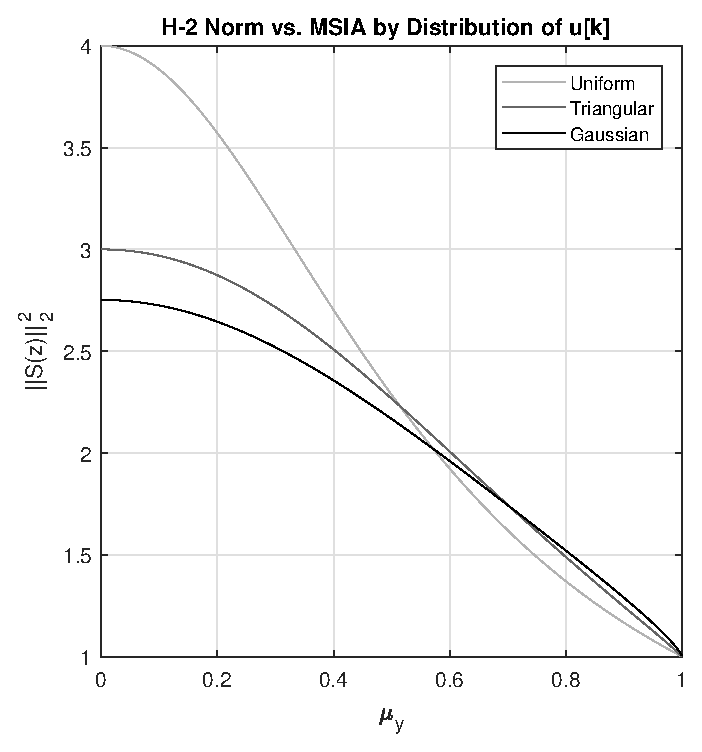
\includegraphics[width=2.5in]{h2-criterion}
	\caption{The choice of \glsentryshort{PDF} for the quantizer input signal places bounds on the squared \gls{H2} norm of the \gls{NTF} for a given \glsentryshort{MSIA} \cite{Risbo1994}.} \label{fig:h2-criterion}
\end{figure}

To employ this stability criterion, the \gls{H2} norm of the sensitivity function, or $r \rightarrow e$ channel of \autoref{eq:aug}, is constrained to a value dependent on the desired \gls{MSIA} $||u||_\infty$ and the choice of \gls{PDF}. This criterion is seen in \autoref{eq:h2} and is only applicable to \gls{DT} designs because the \gls{CT} sensitivity function has infinite \gls{H2} norm.

\begin{equation}
	||G_{er}(z)||_2 \leq \gamma_2. \label{eq:h2}
\end{equation}
 
 \subsection{\gls{l1} Stability Criterion}
 \label{sec:stab-l1}
 
The \gls{l1} stability criterion (also known as Anastassiou's stability criterion) is best understood when the modulator is transformed into the equivalent error feedback structure shown in \autoref{fig:ef-model}. This form is primarily of theoretical importance because its implementation is extremely sensitive to filter coefficient values in the feedback path \cite{Schreier1997}. The advantage for analysis is that the \gls{NTF} and \gls{STF} are shown in independent blocks. This structure is used to define the \gls{l1} norm stability criterion by writing the equations for signals $u$ and $y$ as follows:
 
 \begin{figure}
 	\centering
	% Error Feedback Sigma Delta Modulator
	\begin{tikzpicture}[ampersand replacement=\&,scale=0.75, every node/.style={scale=0.75}]
	
		% Place nodes using a matrix
		\matrix (m1) [row sep=2.5mm, column sep=5mm]
		{
			%------------------------------------------------------------------------------------------------------------------------
			\node[dspnodeopen,dsp/label=left]					(m10) {$r$};				\&
			\node[dspfilter,label={below:$T(\lambda)$}]				(m11) {$\frac{H_0(\lambda)}{1-H_1(\lambda)}$};	\&
			\node[dspadder]								(m12) {};				\&
			\node[coordinate]								(m13) {};				\&
			\node[dspnodefull,label={above:$u$}]					(m14) {};				\&
			\node[dspsquare,label={below:Quantizer}]				(m15) {\RaisingEdge};		\&
			\node[dspnodefull]								(m16) {};				\&
			\node[dspnodeopen,dsp/label=right]					(m17) {$y$};				\& \\
			%------------------------------------------------------------------------------------------------------------------------
			\node[coordinate]								(m20) {};				\&
			\node[coordinate]								(m21) {};				\&
			\node[coordinate]								(m22) {};				\&
			\node[dspfilter,label={below:$S(\lambda) - 1$}]			(m23) {$-\frac{H_1}{1 - H_1}$};	\&
			\node[dspadder,label={above left:$-$}]				(m24) {};				\&
			\node[coordinate]								(m25) {};				\&
			\node[coordinate]								(m26) {};				\& \\
			%------------------------------------------------------------------------------------------------------------------------
		};
	
		%\node[draw,inner xsep=15pt,inner ysep=10pt,dashed,fit={($(m05.north)+(-0.5, 0.7)$) ($(m15.south)+(0.5, -0.6)$)},label={[align=center]below:Linear Model}] {};
	
		\draw[dspconn] 	(m10) -- (m11);
		\draw[dspconn] 	(m11) -- (m12);
		\draw[dspline] 	(m12) -- (m14);
		\draw[dspconn] 	(m14) -- (m15);
		\draw[dspline] 	(m15) -- (m16);
		\draw[dspconn]	(m16) -- (m17);
		\draw[dspline] 	(m16) -- (m26);
		\draw[dspconn] 	(m26) -- (m24);
		\draw[dspconn] 	(m24) -- node[midway,above] {$e$} (m23);
		\draw[dspline] 	(m23) -- (m22);
		\draw[dspconn] 	(m22) -- (m12);
		\draw[dspconn]	(m14) -- (m24);
	
	\end{tikzpicture}
	\caption{The block diagram of the error feedback form of a sigma delta modulator.}  \label{fig:ef-model}
\end{figure}

\begin{align}
	u &= rT(\lambda) + e\left(S(\lambda) - 1\right) \label{eq:l1-u} \\
	y &= e + u \nonumber \\
	&= rT(\lambda) + eS(\lambda). \nonumber
\end{align}

In the time domain, the input to the quantizer from \autoref{eq:l1-u} can be bounded by the following (the \gls{DT} version is shown):

\begin{equation}
	\left|u[k]\right| \leq \left|\sum_{i=1}^{\infty} t[i]r[t - i]\right| + \left|\sum_{i=1}^{\infty} \left(s[i] - 1\right)e[t - i]\right|, \label{eq:l1-bound1}
\end{equation}

where $t[k]$ is the impulse response of the \gls{STF} and $s[k]$ is the impulse response of the \gls{NTF}. Because the \gls{STF} only operates on the input as a pre-filter, the assumption $T(\lambda) = 1$ is taken and \autoref{eq:l1-bound1} simplifes to:

\begin{equation}
	\left|u[k]\right| \leq |r[k]| + \left|\sum_{i=1}^{\infty} \left(s[i] - 1\right)e[t - i]\right|. \label{eq:l1-bound2}
\end{equation}

With a single-bit quantizer, the output $y$ is quantized to $\{-1, 1\}$ so the quantization error signal is bounded to within $\left[0, \frac{\Delta_Q}{2}\right]$ if $\left|u[k]\right| \leq 2$, where \gls{delta} is the quantization step size, in this case 2.

\begin{equation} 
	\left|u[k]\right| \leq |r[k]| + \left|\sum_{i=1}^{\infty} \left(s[i] - 1\right)\right|\frac{\Delta_Q}{2} \label{eq:l1-bound3}
\end{equation}

Taken over all time, the maximum magnitude of each signal is the $\ell_\infty$ norm and the summation over the impulse response of $S(\lambda) - 1$ in Equation \ref{eq:l1-bound3} is its \gls{l1} norm. The \gls{l1} norm is equivalent to the maximum peak-to-peak gain of the system. Substituting this into \autoref{eq:l1-bound3} and simplifying $\frac{\Delta_Q}{2} = 1$ gives:

\begin{align*}
	||u||_\infty &\leq ||r||_\infty + ||S(\lambda) - 1||_1 \\
	&\leq ||r||_\infty + ||S(\lambda)||_1 - 1	.
\end{align*}

Assuming a worst case quantizer input magnitude of $||u||_\infty = 2$, the expression for \gls{l1} stability based on maximum input magnitude is shown in Equation \ref{eq:l1-bound5} \cite{Anastassiou1989}.

\begin{equation} 
	 ||S(\lambda)||_1 \leq 3 - ||r||_\infty \label{eq:l1-bound5}
\end{equation}

Thus, a modulator with a single-bit quantizer is guaranteed to be stable for inputs of magnitude less than three minus the \gls{l1} norm of the NTF. If this value is negative, the modulator is not proven stable by this criterion, for any input. The \gls{l1} criterion is powerful because it is a sufficient condition of \gls{BIBO} stability but it is very conservative as it assumes the worst-case input to the loop filter which may be impossible or extremely unlikely. Like the \gls{H2} and \gls{Hinf} cases, the \gls{l1} stability criterion may be applied to the $r \rightarrow e$ system in \autoref{eq:aug} by the following:

\begin{equation}
	||G_{er}(\lambda)||_1 \leq \gamma_1. \label{eq:l1}
\end{equation}

\subsection{Scale Invariance of the Single-Bit Quantizer}
\label{sec:stab-si}

Here an important result is mentioned that reduces conservatism in the stability criteria from \autoref{sec:stab-h2} and \autoref{sec:stab-l1} that are derived from a norm constraint on the \gls{NTF}. If $K$ is interpreted not a a time-varying gain that models the quantizer but as a fixed design variable, it is obvious that the value of $K$ has no effect if it precedes the single-bit quantizer. The filter $H_1(\lambda)$ in expression for the \gls{NTF} from \autoref{eq:s} may be substituted by the filter and gain in series, yielding:

\begin{equation}
	S(K, \lambda) = \frac{1}{1 - KH_1(\lambda)}. \label{eq:scale-invariance}
\end{equation}

The fictitious gain may be swept in the region $(0, \infty)$ in a nonlinear search to minimize the norm of interest. Because all these \gls{NTF}s are equivalent, the smallest achieved value $\min_K ||S(K, \lambda)||_p$ can be used in place of $||S(\lambda)||_p$ for $p = 1, 2$ as a less conservative stability criterion.

\section{Stability Concepts Not Used by this Optimization Framework}
\label{sec:stab-notused}

It may be worthwhile to introduce further methods of designing sigma delta modulators that are likely stable. The method in this section are presented for a greater understanding of ways to promote stability but are not able to be used in the optimization framework for the reasons provided.

\subsection{Methods Ensuring Bounded States}

A different way of ensuring stability of a modulator system is the positive invariant set approach. This is a mixed analytical and simulation-based method to find positive invariant sets in the state-space of the system. These are regions of \gls{order}-dimensional space for which, once entered, the states of the system $x$ remain inside under given input conditions. The method is computationally intesive and relies on sampling to expand or contract the set bounds \cite{Schreier1997}, which is not rigorous. However, given a random enough input, it may be a very close approximation to the actual positive invariant sets. A simpler version of this technique uses hypercubes as set boundaries and can be combined with the \gls{l1} rule to ensure stability \cite{Yagyu2004a}. The method is a good analysis of predicted stability because it also captures the integrator state values of the system which are important for the actual circuit implementation. However, it is not easy to apply as a design method.

\subsection{Diagonal Modulators}

It is shown in \cite{Steiner1997} that many modulator topologies can be converted into a state-space diagonal representation of the \gls{LF}. In these cases, an \gls{order}th order modulator simplifies into \gls{order} parallel 1st-order modulators interacting only through the quantizer nonlinearity. By examining the stability of the 1st-order modulator using its fixed points \cite{Steiner1996}, the parallel modulators can be shown as a ``shifted'' version, where the shift indicates an offset at the quantizer input due to the other parallel paths. The equations for the fixed points are rearranged to form constraints on the system's poles, inputs, and output matrix coefficients. The downside of this method is that the loop filter is restricted to a specific form and the mathematics become diffcult when complex conjugate poles are introduced as are present in most high-order designs \cite{Mladenov2013}.

\section{Performance Goals}
\label{sec:stab-perf}

The performance goal for the design of sigma delta modulators is simply the attenuation of quantization error in the signal band. In a signals and systems context, this can be made solvable by minimizing the \gls{Hinf} norm of the noise transfer function within the signal band. In the sigma delta literature, this is sometimes called min-max optmization and has some advantages in contrast to minimization of the power using the \gls{H2} norm \cite{Nagahara2012}. To frame the problem, one must first specify a frequency range of interest. In the \gls{DT} case, this is equal to $\frac{\pi}{OSR}$ and in the \gls{CT} case, this is equal to the actual signal band. Using the \gls{GKYP} expression, the \gls{Hinf} norm of the \gls{NTF} in the signal band is minimized to either below a target value (feasibility problem) or as low as possible (optimization problem), subject to any of the above stability constraints. With reference to the augmented system in \autoref{eq:aug}, the \gls{GKYP} constraint is placed on the $r \rightarrow e$ channel that exposes the sensitivity function:

\begin{equation}
	\min_{\lambda \in [\omega_l, \omega_h]} ||G_{er}(\lambda)||_\infty \label{eq:perf}.
\end{equation}

In \gls{DT} designs, the Bode integral (\ref{eq:bodeint-dt}) combined with the performance goal sets the roll-off of the \gls{NTF}. For \gls{CT} designs, the performance goal combined with any stability constraint does not capture the effect of the quantizer sampling frequency because the \gls{S/H} block was omitted in \autoref{sec:in-ctm}. This leads to designs with very low roll-off. To rectify this and force sharp roll-off, the constraint in \ref{eq:ct-constraint-stf} is added for \gls{CT} designs. This forces sharp roll-off by reducing the \gls{Hinf} norm of the complementary sensitivity function (\gls{STF}) just outside the signal band. Because $S(j\omega) + T(j\omega) = 1 \quad \forall \omega$, this constraint allows the sharp roll-off to be optimized for. The appearance of this constraint also shows evidence of the implicit antialiasing feature of \gls{CT} loop filters.

\begin{equation}
	||G_{yr}(j\omega)||_\infty \leq \gamma_{T} \quad \forall \omega \in [\omega_h, f_s] \label{eq:ct-constraint-stf}
\end{equation}